\section{Case-Studies}
TODO: emphasise different types of games/simulations: need to be very clear of the difference between the 2 games
TODO: experimentation description: which language, with which model, with which configuration, number of agents, number of replications,...
TODO: what about language-differences, which language did we use?

In this section we revisit the Prisoners Dilemma model of \cite{nowak_evolutionary_1992} and present the Heroes \& Cowards model of \cite{wilensky_introduction_2015} and show results simulating both with the four update-strategies. 

TODO: why 25\% heroes, why this big number of agents 100.000?

TODO: what do I want to achieve with this test? it is basically to show 1st: that only the parallel-strategy produces the results which match the ones of the original paper in the prisoners dilemma, 2nd: that the other update-strategies create completely different results, 3rd: the heroes \& cowards game seems to be unaffected by different update-strategies.

\subsection{Effect of using different Update-Strategies}

\begin{table*}[t]
	\begin{tabular}{c c c}
		& Prisoners Dilemma & Heroes \& Cowards \\ 

		\textit{\rotatebox{90}{sequential strategy}}
		&
		\begin{subfigure}[b]{0.4\textwidth}
			\centering
			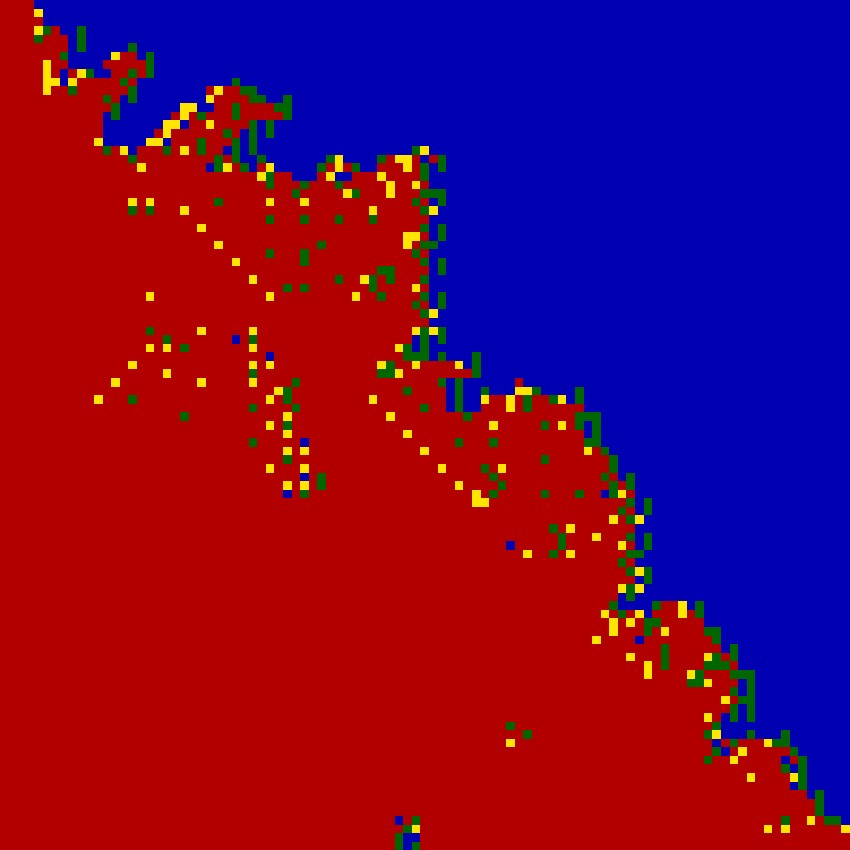
\includegraphics[width=.7\textwidth, angle=0]{./fig/seq_99x99_436steps_MSG_haskell.png}
			\caption{}
			\label{fig:pd_seq}
		\end{subfigure}
    	&
		\begin{subfigure}[b]{0.4\textwidth}
			\centering
			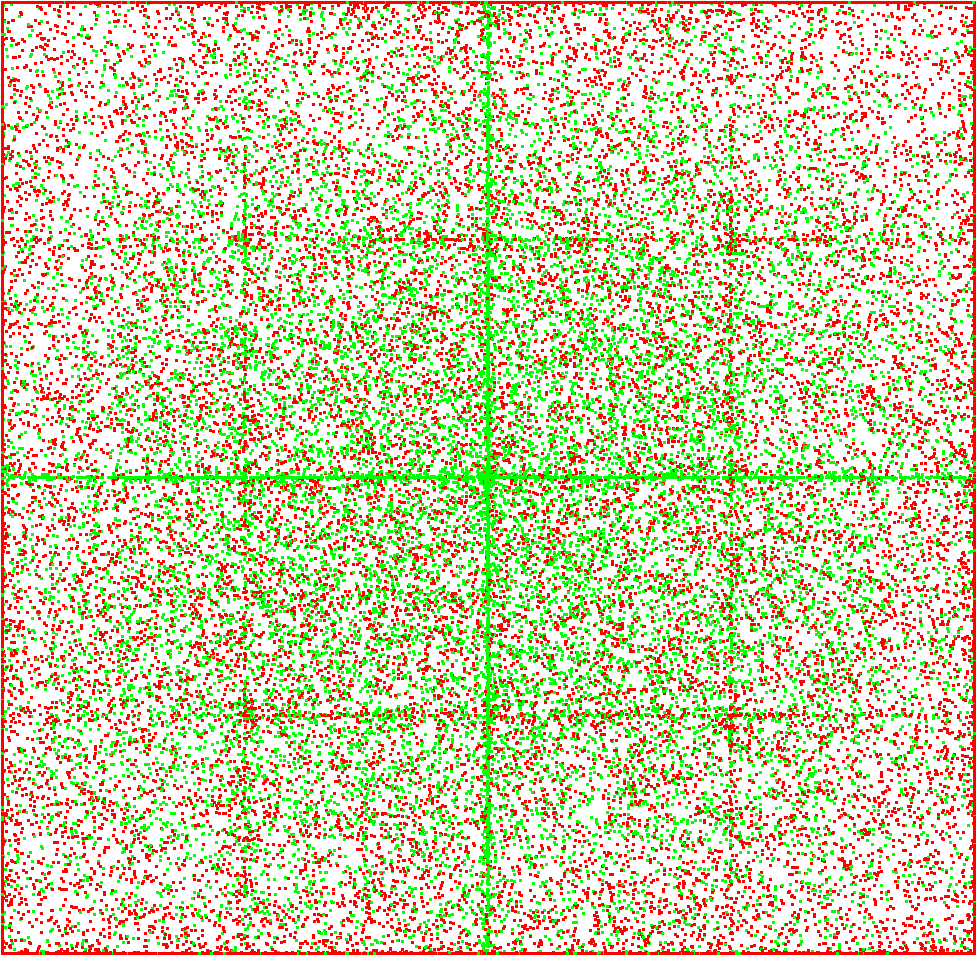
\includegraphics[width=.7\textwidth, angle=0]{./fig/seq_HAC_100_000_500steps_java.png}
			\caption{}
			\label{fig:hac_seq}
		\end{subfigure}
    	\\
    	
    	\textit{\rotatebox{90}{parallel strategy}}
		&
		\begin{subfigure}[b]{0.4\textwidth}
			\centering
			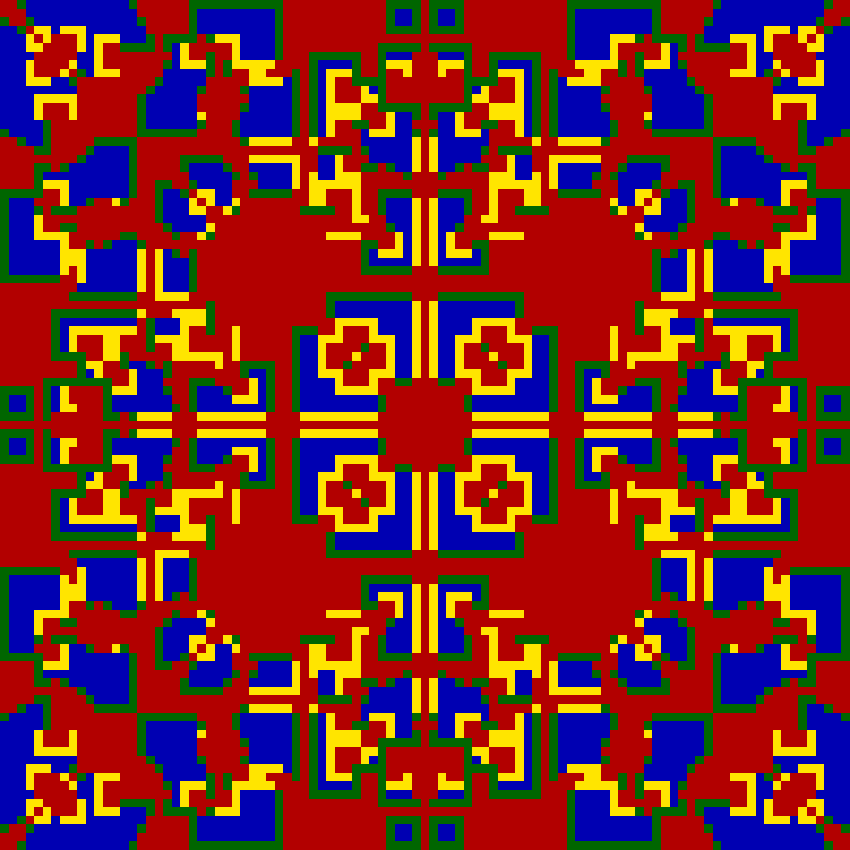
\includegraphics[width=.7\textwidth, angle=0]{./fig/par_99x99_436steps_MSG_haskell.png}
			\caption{}
			\label{fig:pd_par}
		\end{subfigure}
    	&
		\begin{subfigure}[b]{0.4\textwidth}
			\centering
			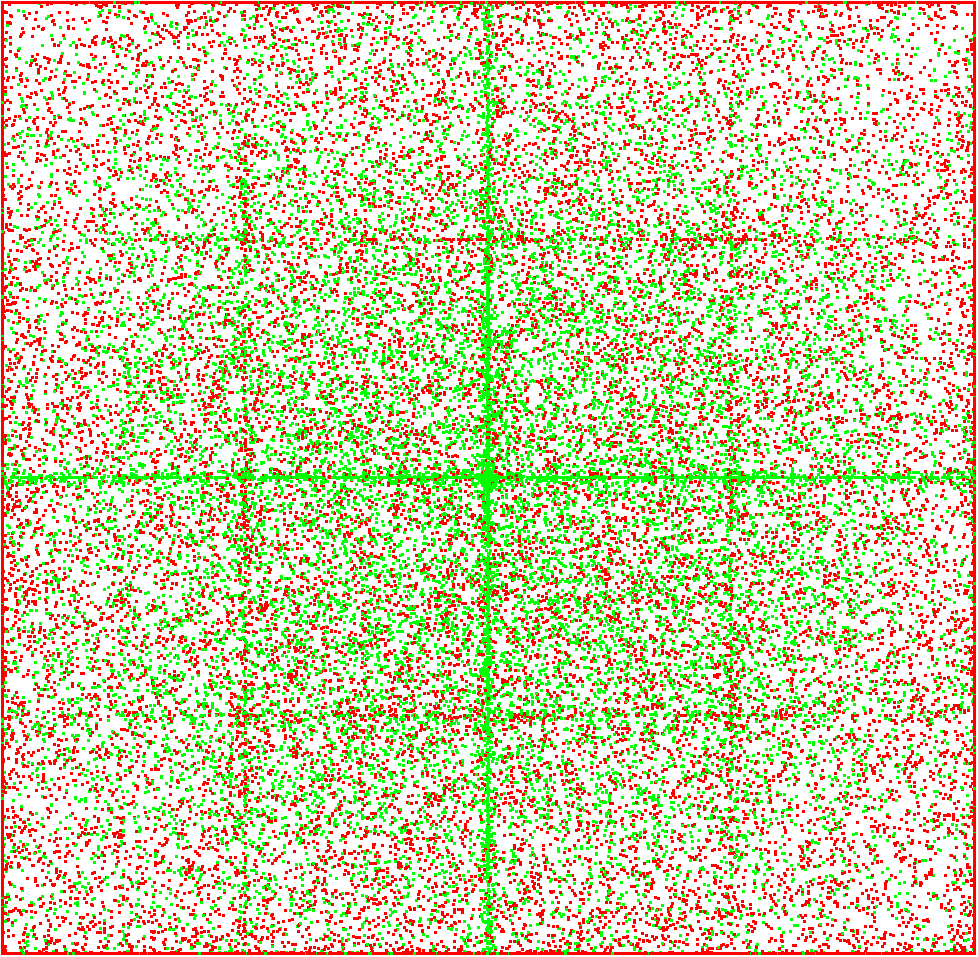
\includegraphics[width=.7\textwidth, angle=0]{./fig/par_HAC_100_000_500steps_java.png}
			\caption{}
			\label{fig:hac_par}
		\end{subfigure}
    	\\
    	
    	\textit{\rotatebox{90}{concurrent strategy}}
		&
		\begin{subfigure}[b]{0.4\textwidth}
			\centering
			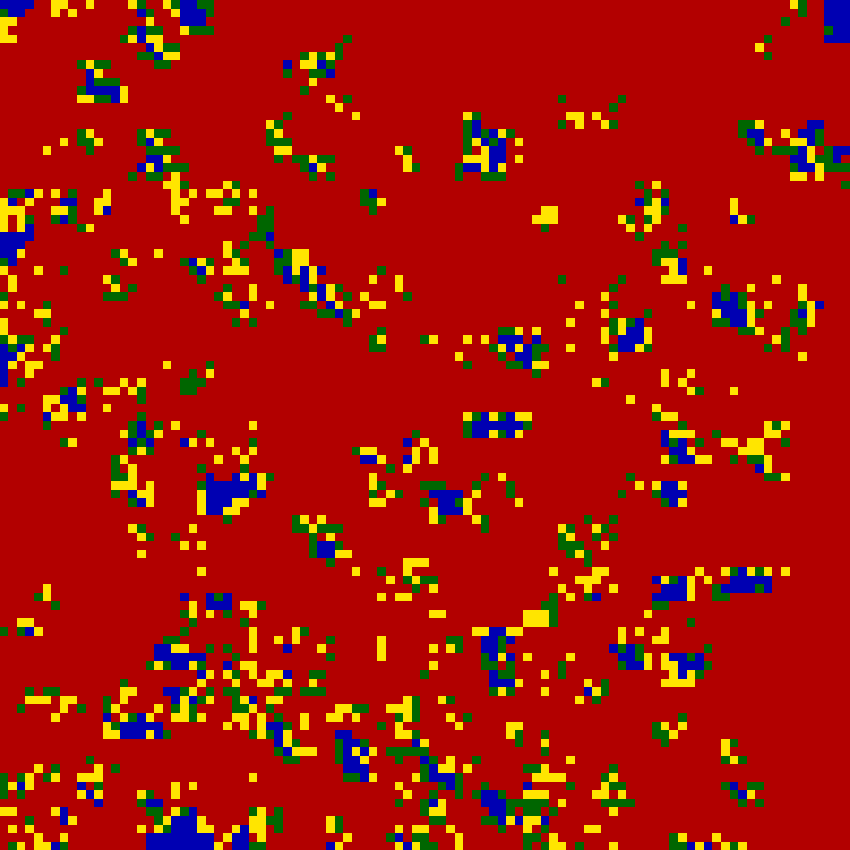
\includegraphics[width=.7\textwidth, angle=0]{./fig/con_99x99_436steps_MSG_haskell.png}
			\caption{}
			\label{fig:pd_con}
		\end{subfigure}
    	&
		\begin{subfigure}[b]{0.4\textwidth}
			\centering
			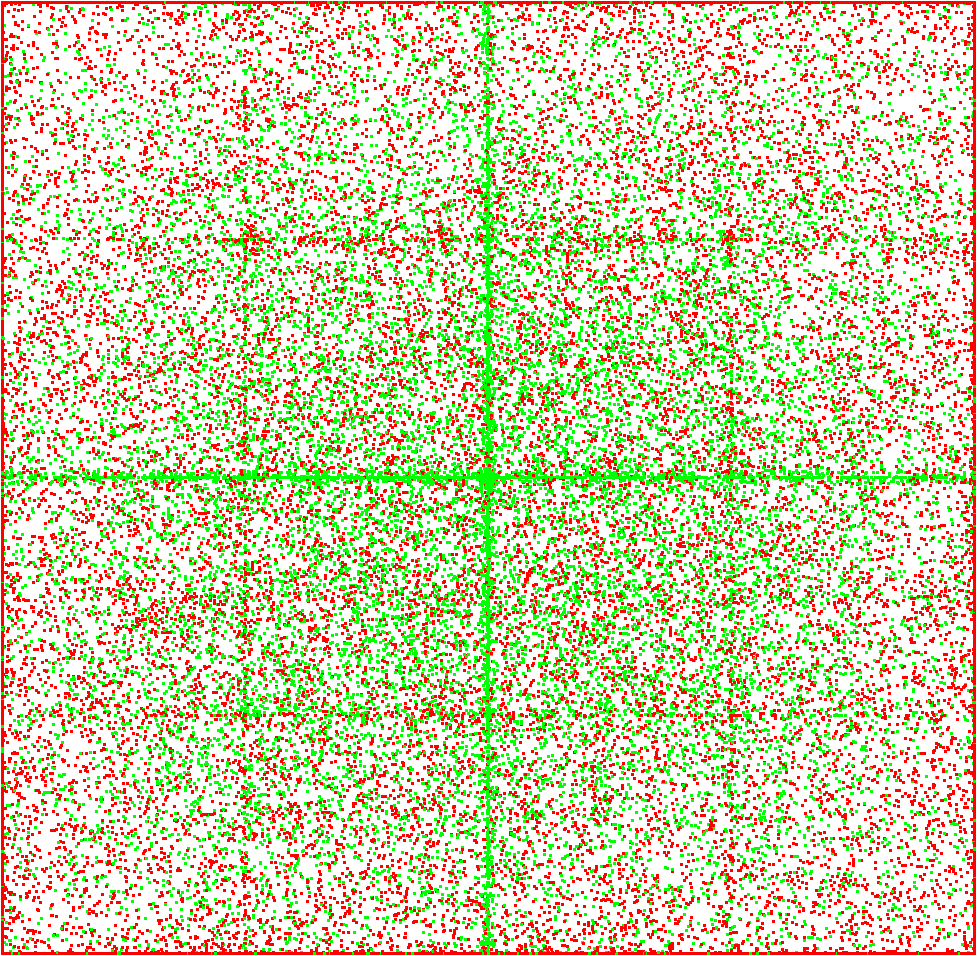
\includegraphics[width=.7\textwidth, angle=0]{./fig/con_HAC_100_000_500steps_java.png}
			\caption{}
			\label{fig:hac_con}
		\end{subfigure}
    	\\ 
    	
    	\textit{\rotatebox{90}{actor strategy}}
		&
		\begin{subfigure}[b]{0.4\textwidth}
			\centering
			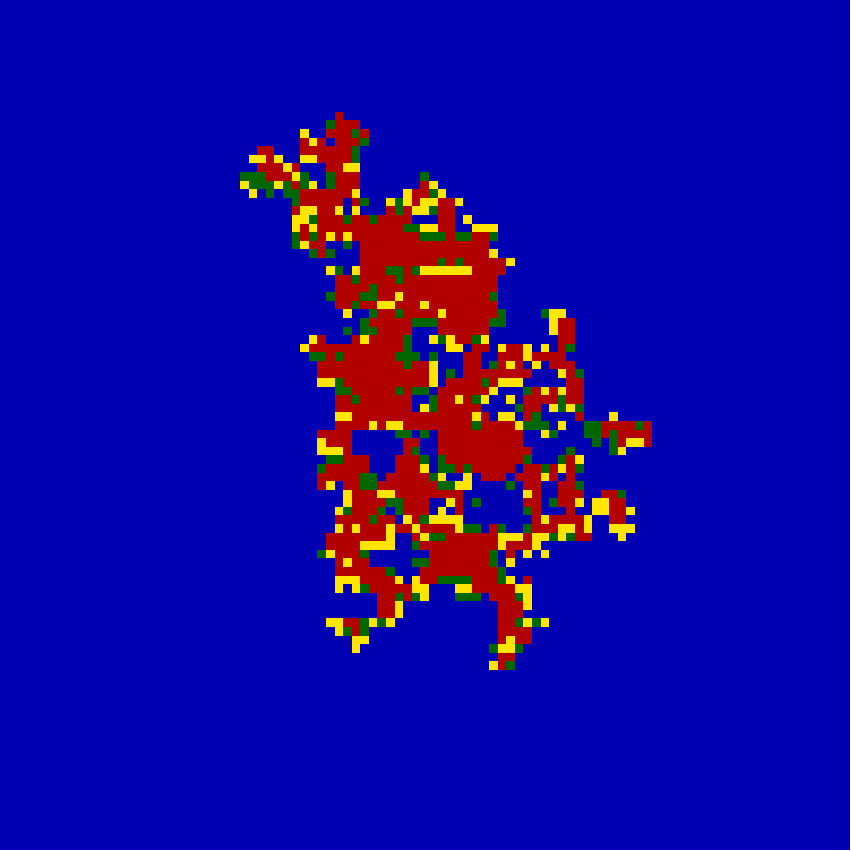
\includegraphics[width=.7\textwidth, angle=0]{./fig/act_99x99_436steps_MSG_haskell.png}
			\caption{}
			\label{fig:pd_act}
		\end{subfigure}
    	&
    	% TODO: this the same picture as in concurrent version from java, put in actor-version generated by scala    
		\begin{subfigure}[b]{0.4\textwidth}
			\centering
			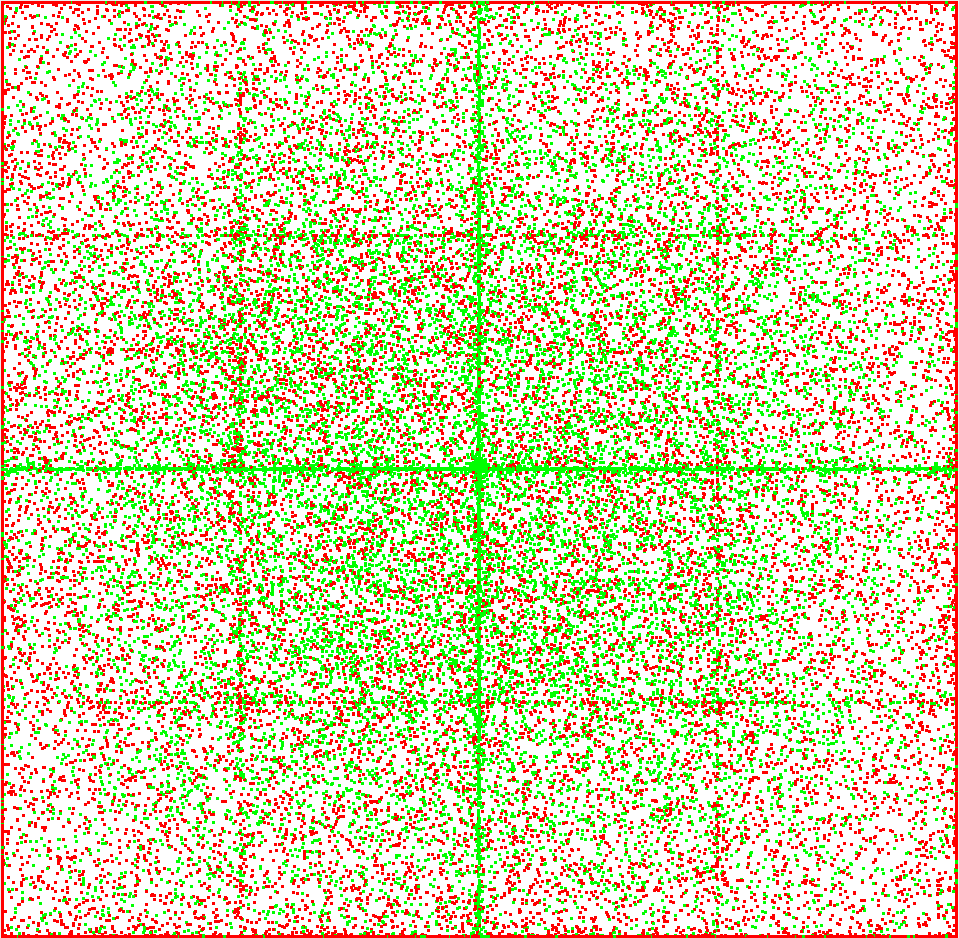
\includegraphics[width=.7\textwidth, angle=0]{./fig/act_HAC_100_000_500steps_scala.png}
			\caption{}
			\label{fig:hac_act}
		\end{subfigure}
    	\\ \hline
	\end{tabular}
	
	\caption{\small Results of Prisoners Dilemma and Heroes \& Cowards with all four update-strategies.} 
	\label{fig:results}
\end{table*}

%\begin{figure*}
%
%	 \centering
	
%    \begin{subfigure}[b]{0.4\textwidth}
%			\centering
%       	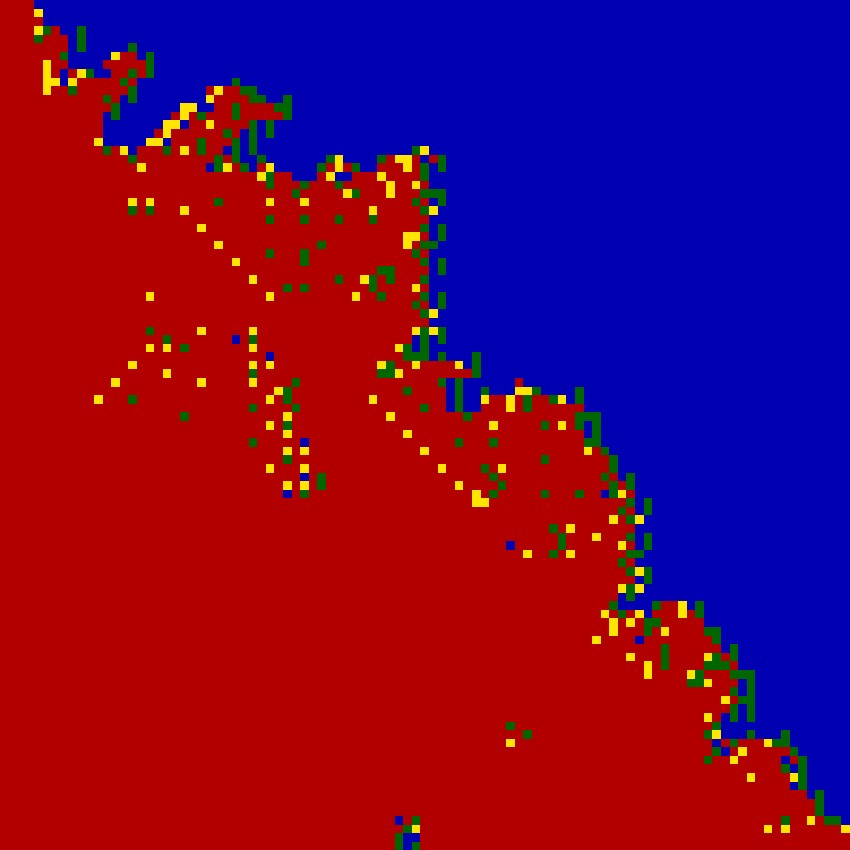
\includegraphics[width=.7\textwidth, angle=0]{./fig/seq_99x99_436steps_MSG_haskell.png}
%        \caption{\textit{sequential} Prisoners Dilemma}
%        \label{fig:pd_seq}
%    \end{subfigure}
%    \begin{subfigure}[b]{0.4\textwidth}
%		\centering
%        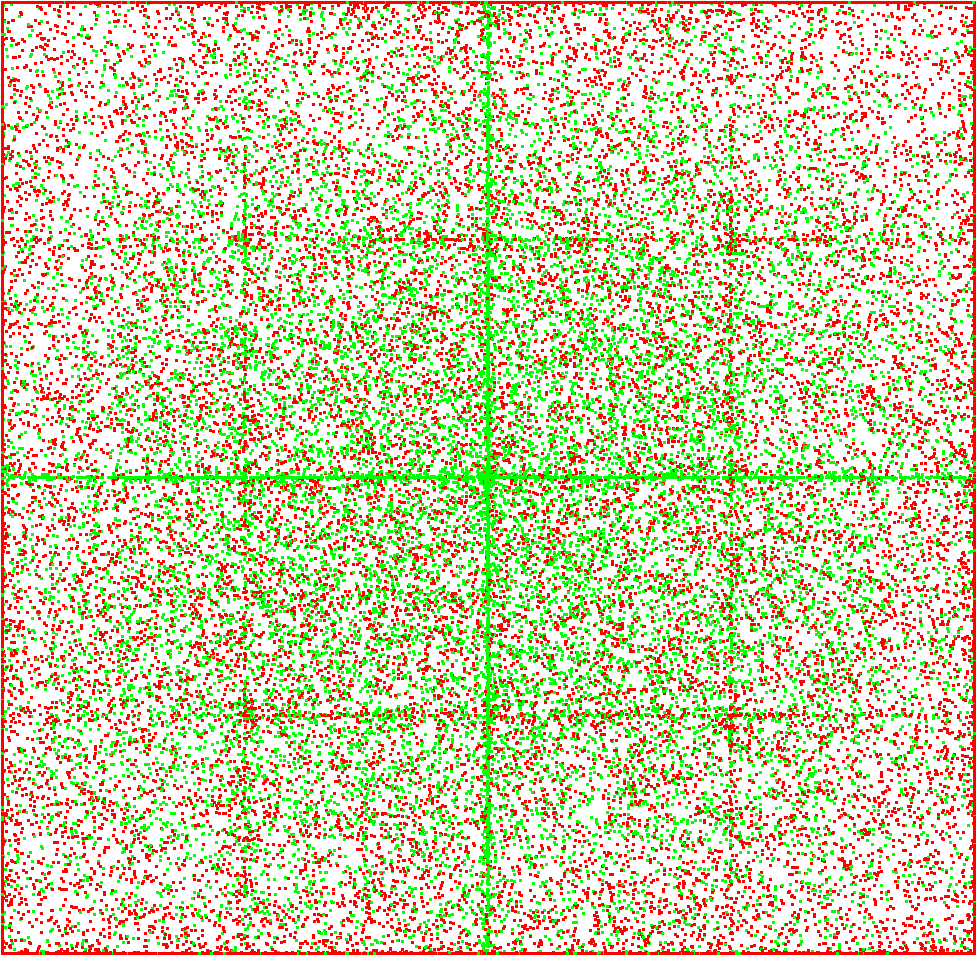
\includegraphics[width=.7\textwidth, angle=0]{./fig/seq_HAC_100_000_500steps_java.png}
%        \caption{\textit{sequential} Heroes \& Cowards}
%        \label{fig:hac_seq}
%    \end{subfigure}
%       

%    \begin{subfigure}[b]{0.4\textwidth}
%		\centering
%       	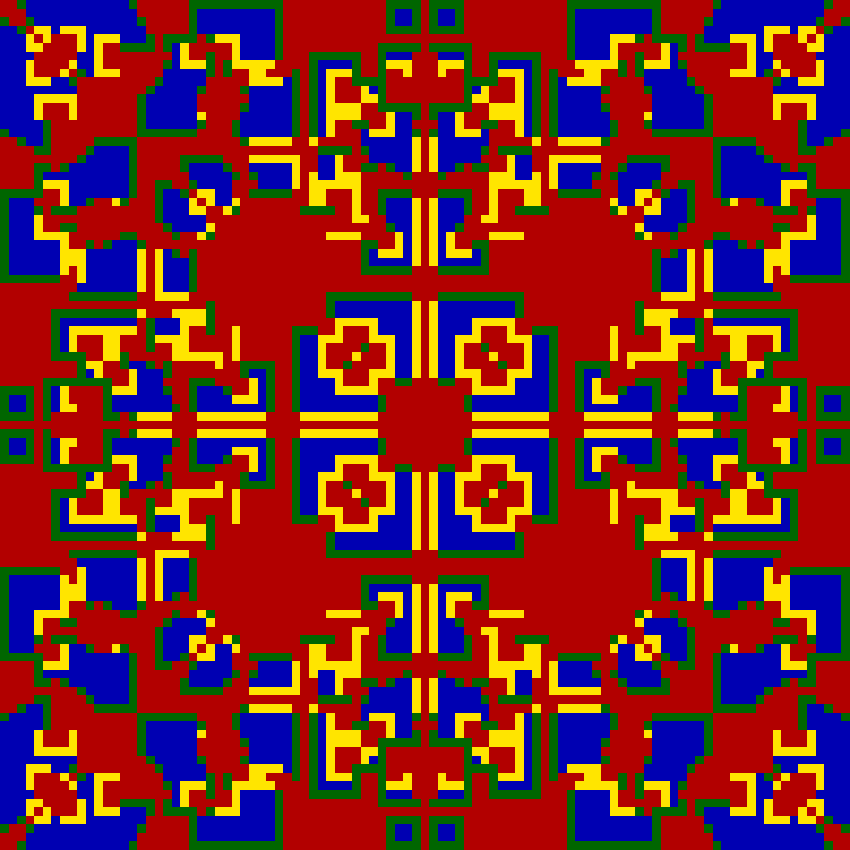
\includegraphics[width=.7\textwidth, angle=0]{./fig/par_99x99_436steps_MSG_haskell.png}
%        \caption{\textit{parallel} Prisoners Dilemma}
%        \label{fig:pd_par}
%    \end{subfigure}
%    \begin{subfigure}[b]{0.4\textwidth}
%    	\centering
%        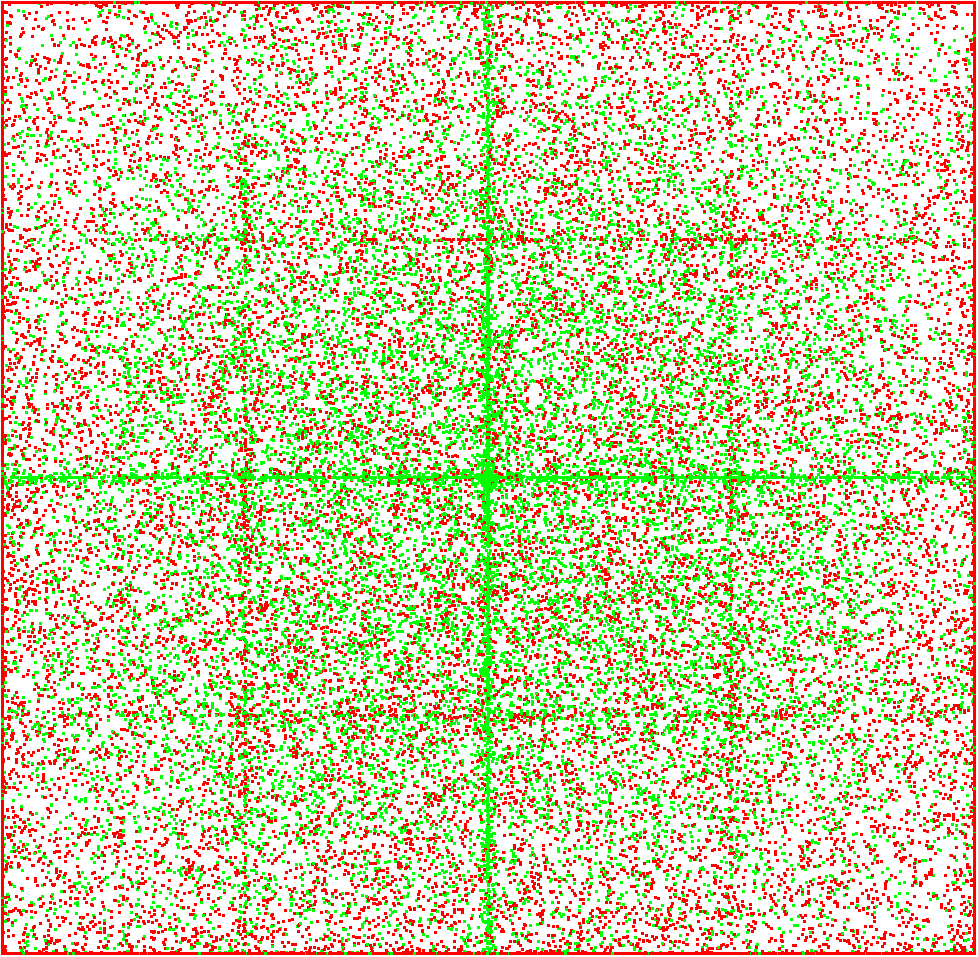
\includegraphics[width=.7\textwidth, angle=0]{./fig/par_HAC_100_000_500steps_java.png}
%        \caption{\textit{parallel} Heroes \& Cowards}
%        \label{fig:hac_par}
%    \end{subfigure}
%        
%
%    \begin{subfigure}[b]{0.4\textwidth}
%		\centering
%       	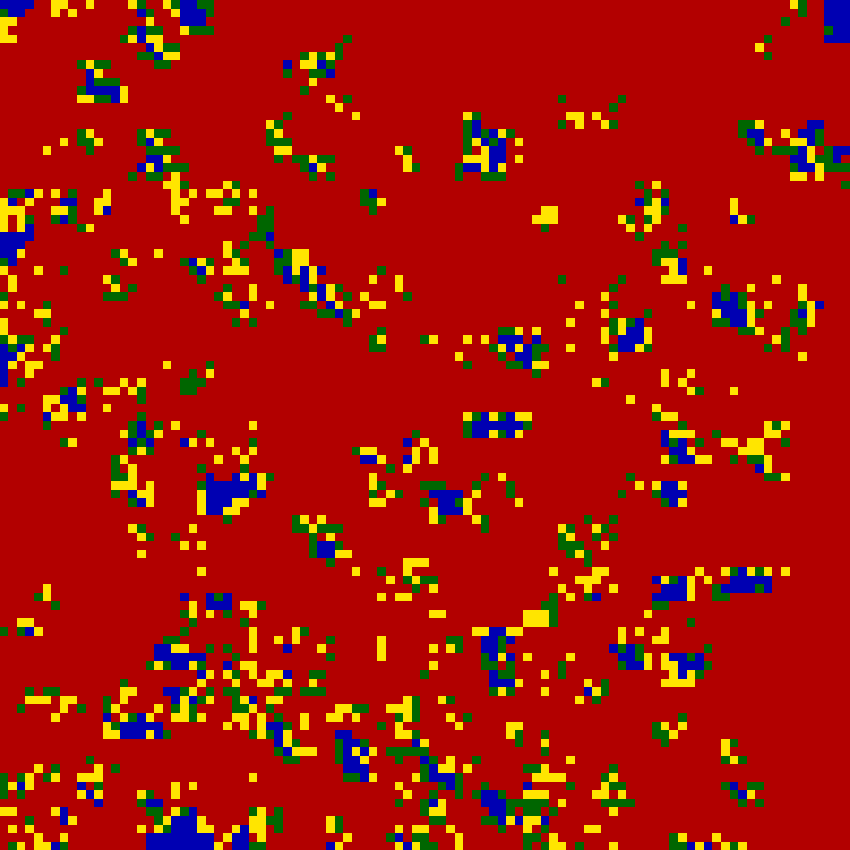
\includegraphics[width=.7\textwidth, angle=0]{./fig/con_99x99_436steps_MSG_haskell.png}
%        \caption{\textit{concurrent} Prisoners Dilemma}
%        \label{fig:pd_con}
%    \end{subfigure}
%    \begin{subfigure}[b]{0.4\textwidth}
%    	\centering
%        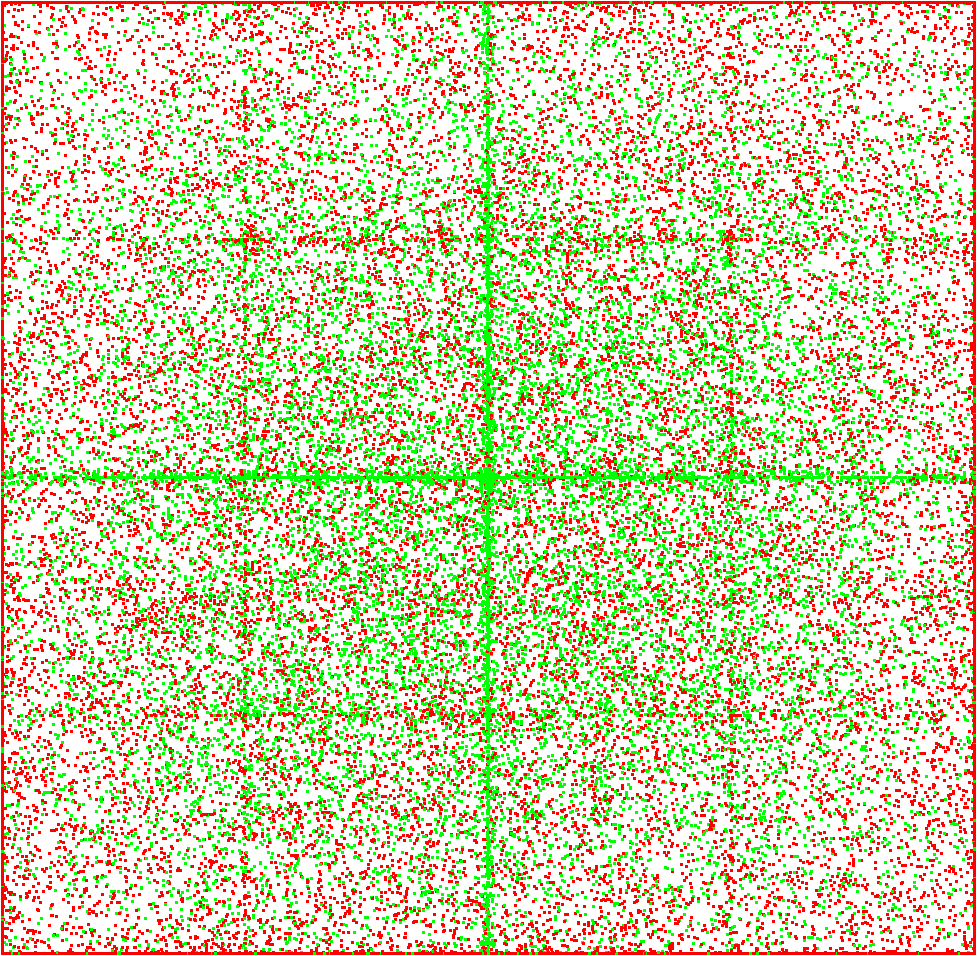
\includegraphics[width=.7\textwidth, angle=0]{./fig/con_HAC_100_000_500steps_java.png}
%        \caption{\textit{concurrent} Heroes \& Cowards}
%        \label{fig:hac_con}
%    \end{subfigure}
%
%
%    \begin{subfigure}[b]{0.4\textwidth}
%		\centering
%       	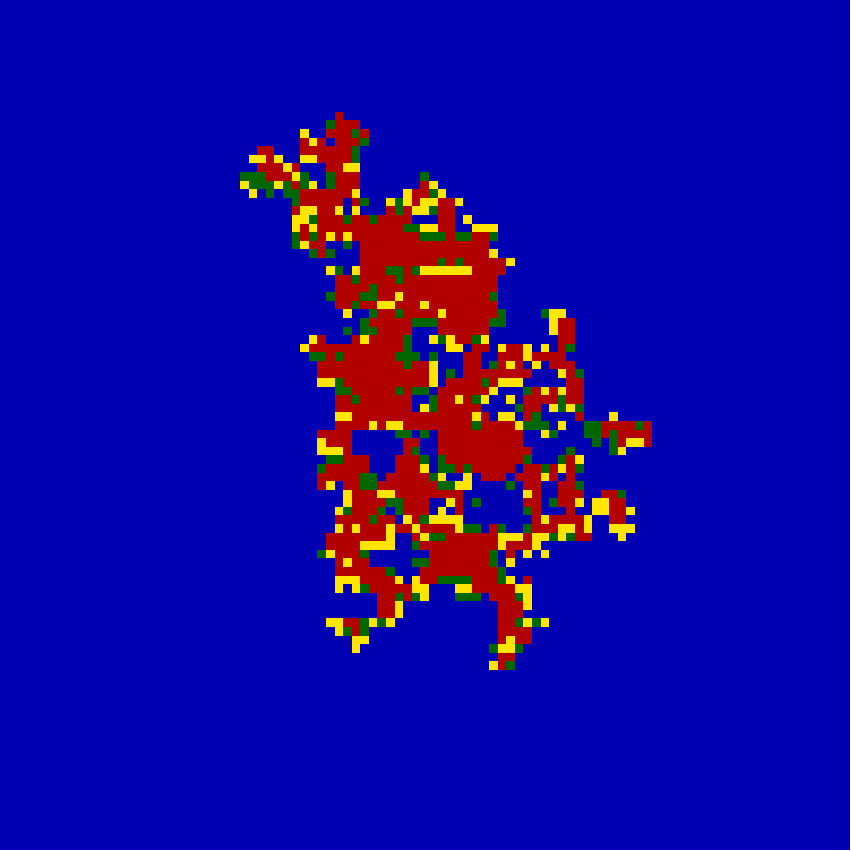
\includegraphics[width=.7\textwidth, angle=0]{./fig/act_99x99_436steps_MSG_haskell.png}
%        \caption{\textit{actor} Prisoners Dilemma}
%        \label{fig:pd_act}
%    \end{subfigure}  
%    \begin{subfigure}[b]{0.4\textwidth}
%    	\centering
%        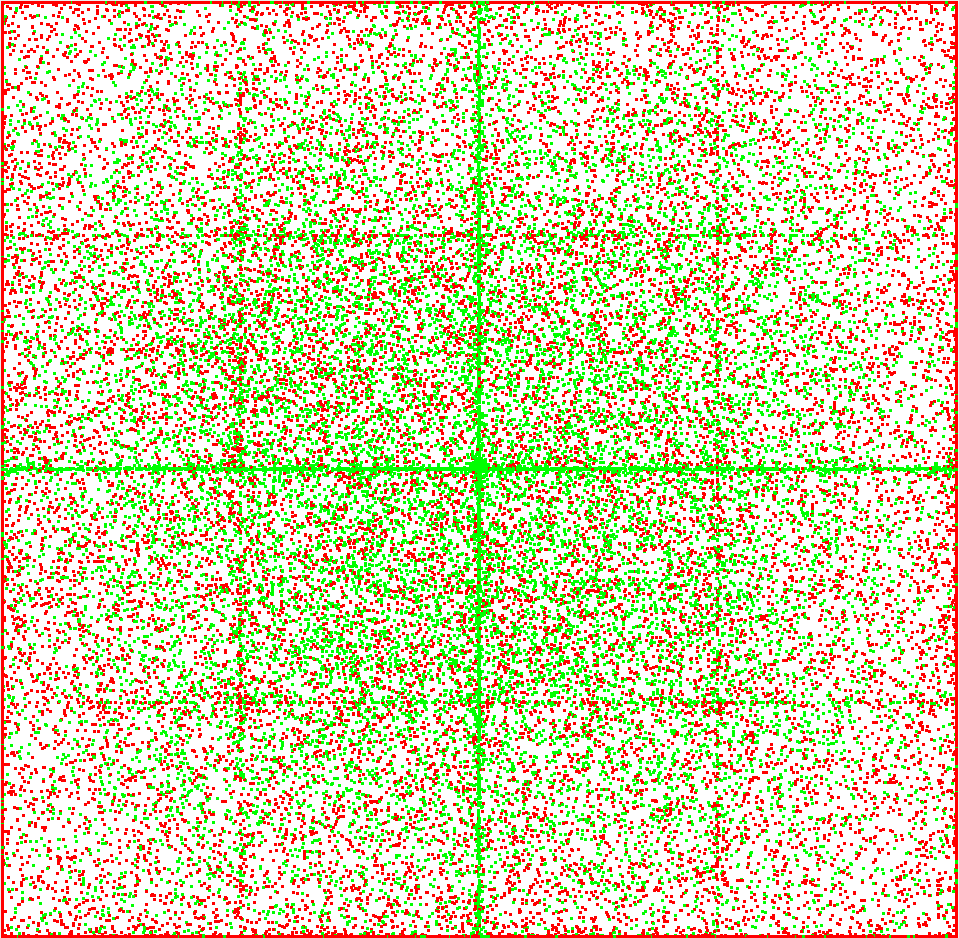
\includegraphics[width=.7\textwidth, angle=0]{./fig/act_HAC_100_000_500steps_scala.png}
%        \caption{\textit{actor} Heroes \& Cowards}
%        \label{fig:hac_act}
%    \end{subfigure}
% TODO: this the same picture as in concurrent version from java, put in actor-version generated by scala    
% TODO: this the same picture as in concurrent version from java, put in actor-version generated by scala    
% TODO: this the same picture as in concurrent version from java, put in actor-version generated by scala    
% TODO: this the same picture as in concurrent version from java, put in actor-version generated by scala    
% TODO: this the same picture as in concurrent version from java, put in actor-version generated by scala    
% TODO: this the same picture as in concurrent version from java, put in actor-version generated by scala  

%	\caption{\small Results of Prisoners Dilemma and Heroes \& Cowards with all four update-strategies.} 
%	\label{fig:results}
%\end{figure*}

When looking at figure \ref{fig:results} the update-strategy which reflects the semantics of the model is the Parallel Strategy as all others clearly fail to reproduce the pattern as shown by the results in the original paper TODO: in figure \ref{fig:sync_patterns}. We can imply that only the Parallel Strategy is suitable to simulate this model because only that strategy is the one which renders the results of the original paper, meaning it is the 'correct' strategy. \\
The reason why the others fail to reproduce the pattern is due to the non-parallel and unsynchronized way that information spreads through the grid. In the Sequential Strategy the agents further ahead in the queue play the game earlier and influence the neighbourhood so agents in the neighbourhood which play the game later experience an already changed environment and  messages in their queue and act differently based upon these informations. This is not the case in the Parallel version where all agents play the game on the frozen state of the previous step and the outcome of each agents game will only be visible in the next step. In the Concurrent and Actor Strategy the agents run in parallel but changes are visible immediately and concurrently, leading to the same non-structural patterns as in the Sequential Strategy. \\
Note that the Concurrent and Actor Strategy produce different results on every run due to the inherent non-deterministic event-ordering introduce by concurrency. Also note that it is not possible to calculate 45 steps for the Actor Strategy as it lacks the Global Synchronization property. To arrive at a relative comparative result we just waited until the first agent arrives at a local time of 45 and then rendered the result. 

\subsection{Heroes \& Cowards}
Although the individual agent-positions of runs with the same configuration differ between update-strategies we experienced the forming of the emergent cross-pattern as seen in figure \ref{fig:results} in all four update-strategies. We can conclude that the Heroes \& Cowards model seems to be more robust to the selection of its update-strategy and that its emergent property - the formation of the cross - is stable under differing update-strategies. One would not see a difference between the different strategies so only one picture was included. Note that to test the Actor Strategy with a this high number of agents we used our implementation in Scala with Actors as Java is not able to have this high number of threads and our Haskell implementation suffers from performance issues, resorting to Scala with Actors. The results were nearly the same there, showing the big green emergent cross-pattern in the center but lacking the smaller red crosses in each section, something we attribute to the local-time of each agent and the relativity of observing the simulation.